% ============================================================================
% Course Wrap-Up and Outlook
% Duration: 25 minutes
% ============================================================================

\documentclass[aspectratio=169,11pt]{beamer}

% ---------- Theme and colors ----------
\usecolortheme{dove}
\setbeamertemplate{navigation symbols}{}
\setbeamertemplate{footline}{%
  \hfill\usebeamerfont{page number in head/foot}%
  \usebeamercolor[fg]{normal text}%
  \insertframenumber\,/\,\inserttotalframenumber\kern1em\vskip4pt}
\setbeamerfont{frametitle}{size=\huge}

% ---------- Packages ----------
\usepackage[utf8]{inputenc}
\usepackage[T1]{fontenc}
\usepackage{amsmath,amssymb,amsfonts}
\usepackage{bm}
\usepackage{graphicx}
\graphicspath{{fig/}}
\usepackage{tikz}
\usetikzlibrary{shapes,arrows.meta,positioning,calc,fit,backgrounds,patterns,decorations.pathreplacing}
\usepackage{booktabs}
\usepackage{hyperref}
\usepackage{xcolor}

% ---------- Custom colors ----------
\definecolor{uzhblue}{rgb}{0,0,0.5}
\definecolor{uzhgreylight}{RGB}{236,238,241}
\definecolor{uzhgreydark}{RGB}{81,86,94}
\definecolor{harvardcrimson}{RGB}{153,0,0}
\definecolor{unil@blue}{RGB}{0,140,204}
\definecolor{unil@black}{RGB}{35,31,32}
\definecolor{darkgreen}{RGB}{0,100,0}
\definecolor{darkred}{RGB}{139,0,0}
\definecolor{softblue}{RGB}{70,130,180}
\definecolor{softorange}{RGB}{230,159,0}
\definecolor{softgreen}{RGB}{0,158,115}

% ---------- Set beamer colors ----------
\setbeamercolor{frametitle}{bg=uzhgreylight, fg=uzhblue}
\setbeamercolor{title}{fg=uzhblue}
\setbeamercolor{structure}{fg=uzhblue}
\setbeamercolor{block title}{bg=unil@blue, fg=white}
\setbeamercolor{block body}{bg=uzhgreylight}
\setbeamercolor{block title alerted}{bg=darkred,fg=white}
\setbeamercolor{block body alerted}{bg=red!5}
\setbeamercolor{block title example}{bg=darkgreen,fg=white}
\setbeamercolor{block body example}{bg=green!5}
\setbeamercolor{item}{fg=unil@black}
\setbeamercolor{normal text}{fg=unil@black}

% ---------- Emphasis and hyperlinks ----------
\newcommand{\emphc}[1]{\textcolor{harvardcrimson}{#1}}
\hypersetup{colorlinks,linkcolor=harvardcrimson,urlcolor=harvardcrimson}

% ---------- Math commands ----------
\newcommand{\R}{\mathbb{R}}
\newcommand{\E}[1]{\mathbb{E}\!\left[#1\right]}

% ---------- Title ----------
\title[Deep Learning for Dynamic Economic Models]
{Deep Learning for Economics and Finance}
\subtitle{Key takeaways, method choice, and outlook}
\author{Simon Scheidegger}
\institute[HEC Lausanne]{HEC, University of Lausanne}
\date{}

\begin{document}

% --- Slide 1: Title ---
{\setbeamercolor{background canvas}{bg=uzhgreylight}
\begin{frame}
\titlepage
\vspace{-0.4cm}
\begin{center}
{\footnotesize Closing lecture: synthesis, method choice, and outlook}\\[4pt]
{\footnotesize Materials: \url{https://github.com/sischei/Deep_Learning_for_Solving_And_Estimating_Dynamic_Economic_Models}}
\end{center}
\end{frame}
}

% --- Slide 2: Wrap-up roadmap ---
\begin{frame}{Wrap-Up Roadmap}
\begin{enumerate}
    \item \textbf{Synthesis of the full course pipeline}
    \item \textbf{Decision guide: DEQN, PINN, Surrogates, GP}
    \item \textbf{Climate-policy lessons}
    \item \textbf{Implementation checklist and outlook}
\end{enumerate}
\end{frame}

% --- Learning objectives ---
\begin{frame}{Learning objectives}
\textbf{By the end of the course you should be able to:}
\begin{itemize}
  \item Choose between DEQN, PINN, deep surrogates, and GP+BAL based on problem structure and scalability
  \item Design residual-loss functions that embed economic and climate equations for end-to-end equilibrium learning
  \item Articulate when to include parameters as pseudo-states versus solving repeatedly
  \item Evaluate whether a trained surrogate meets publication standards through residual diagnostics and stress tests
  \item Synthesize deep learning, uncertainty quantification, and constrained optimization for evidence-based policy design
\end{itemize}
\end{frame}


% --- Slide 3: Big picture ---
\begin{frame}{The Big Picture: One Computational Paradigm}
\begin{center}
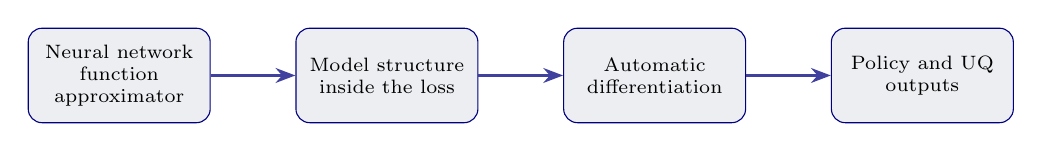
\begin{tikzpicture}[
    box/.style={rectangle, draw=uzhblue, fill=uzhgreylight, rounded corners=5pt,
                text width=2.1cm, minimum height=1.2cm, align=center, font=\scriptsize,
                inner sep=3pt},
    arr/.style={-{Stealth[length=2.5mm]}, very thick, uzhblue!75}
]
\node[box] (nn)     at (0,0)    {Neural network\\function approximator};
\node[box] (loss)   at (3.4,0)  {Model structure\\inside the loss};
\node[box] (ad)     at (6.8,0)  {Automatic\\differentiation};
\node[box] (policy) at (10.2,0) {Policy and UQ\\outputs};

\draw[arr] (nn.east)   -- (loss.west);
\draw[arr] (loss.east) -- (ad.west);
\draw[arr] (ad.east)   -- (policy.west);
\end{tikzpicture}
\end{center}

\vspace{0.25cm}
\begin{block}{Across methods}
DEQN, PINN, deep surrogates, and GP-BAL differ in objective and geometry,\\
but share the same core optimization logic.
\end{block}
\end{frame}

% --- Slide 4: Course arc ---
\begin{frame}{Course Arc}
\small
\begin{center}
\begin{tabular}{ll}
\toprule
\textbf{Day} & \textbf{Core step in the pipeline} \\
\midrule
1 & Deep learning foundations and optimization diagnostics \\
2--4 & DEQNs for discrete-time equilibrium (RA, IRBC) \\
5 & Heterogeneous agents, OLG, and Young's method (sequence space, Krusell--Smith) \\
6 & PINNs for continuous-time PDE problems \\
7 & Deep surrogates and GP/BAL for fast policy/estimation loops \\
8 & Climate IAMs, deep UQ, constrained policy design \\
\bottomrule
\end{tabular}
\end{center}

\vspace{0.2cm}
\begin{alertblock}{Main message}
The toolkit is modular: solve, emulate, quantify uncertainty, then optimize policy under explicit constraints.
\end{alertblock}
\end{frame}

% --- Slide 4b: Visual course timeline ---
\begin{frame}{Visual Timeline of the Course Workflow}
\begin{center}
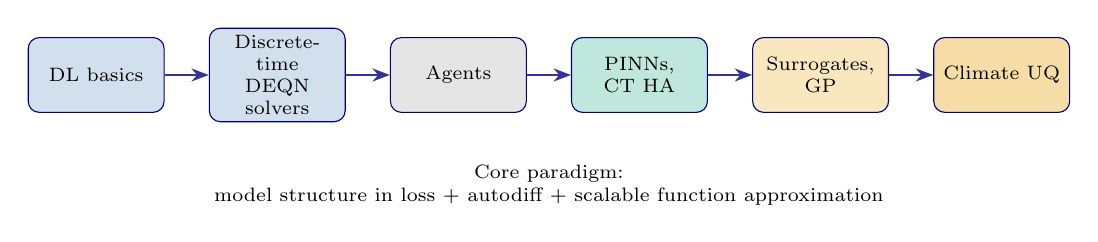
\begin{tikzpicture}[
    phasebox/.style={rectangle, draw=uzhblue, rounded corners=4pt, text width=1.55cm,
                 minimum height=0.95cm, align=center, fill=uzhgreylight, font=\scriptsize,
                 inner sep=2.5pt},
    arr/.style={-{Stealth[length=2.2mm]}, thick, uzhblue!80}
]
\node[phasebox, fill=softblue!25]   (d1) at (0,0)    {DL basics};
\node[phasebox, fill=softblue!25]   (d2) at (2.3,0)  {Discrete-time\\DEQN solvers};
\node[phasebox, fill=gray!20]       (d5) at (4.6,0)  {Agents};
\node[phasebox, fill=softgreen!25]  (d6) at (6.9,0)  {PINNs, CT HA};
\node[phasebox, fill=softorange!25] (d7) at (9.2,0)  {Surrogates, GP};
\node[phasebox, fill=softorange!35] (d8) at (11.5,0) {Climate UQ};

\draw[arr] (d1.east) -- (d2.west);
\draw[arr] (d2.east) -- (d5.west);
\draw[arr] (d5.east) -- (d6.west);
\draw[arr] (d6.east) -- (d7.west);
\draw[arr] (d7.east) -- (d8.west);

\node[font=\scriptsize, align=center] at (5.75,-1.4) {Core paradigm:\\model structure in loss + autodiff + scalable function approximation};
\end{tikzpicture}
\end{center}
\end{frame}

% --- Slide 5: Method decision guide ---
\begin{frame}{Decision Guide: Which Method When?}
\scriptsize
\begin{center}
\begin{tabular}{p{0.16\textwidth}p{0.30\textwidth}p{0.30\textwidth}}
\toprule
\textbf{Method} & \textbf{Use case} & \textbf{Strength} \\
\midrule
DEQN & Discrete-time equilibrium systems & Scales to high-dimensional states \\
PINN & Continuous-time PDE/HJB/KFE systems & Mesh-free PDE residual training \\
Deep surrogate & Repeated model evaluations & Very fast policy and estimation loops \\
GP + BAL & UQ and active design & Built-in uncertainty and sample efficiency \\
\bottomrule
\end{tabular}
\end{center}
\end{frame}

% --- Slide 5b: Brock--Mirman through every lens (mirrors script Tbl 12.2) ---
\begin{frame}{Brock--Mirman Through Every Lens}
\scriptsize
\begin{center}
\begin{tabular}{p{0.13\textwidth}p{0.27\textwidth}p{0.30\textwidth}p{0.18\textwidth}}
\toprule
\textbf{Method} & \textbf{What is approximated} & \textbf{Loss / objective} & \textbf{Diagnostic} \\
\midrule
DEQN              & Savings share $s(K,z)\in(0,1)$              & Squared rel.\ Euler residual on simulated trajectory & $s\to\alpha\beta$ at $\delta=1$, log utility \\
PINN              & Value function $\hat V(a)$, 1-D interval     & HJB residual $\rho V-\max_c[u(c)+V'(a)(ra-c)]$ & $\hat V$ matches CRRA closed form \\
GP + BAL          & $\hat V(K)$ on BM ergodic set                & GP marginal likelihood; BAL picks next $K_*$ & 95\% pred.\ band covers true $V$ \\
SMM + surrogate   & Policy $s(K,z,\varrho)$ pseudo-state on $\varrho$ & SMM moment objective in $\varrho$ & $\hat\varrho$ within MCSE of truth \\
\bottomrule
\end{tabular}
\end{center}

\vspace{0.15cm}
\footnotesize
One model, four lenses. The economic content is identical; the methodology determines what is approximated and what diagnostic certifies convergence.  Companion notebooks in L03, L11, L14, L15.
\end{frame}

% --- Slide 5c: When NOT to use deep learning (mirrors script Sec 12.6) ---
\begin{frame}{When \emph{Not} to Use Deep Learning}
\small
\begin{itemize}
    \item \textbf{State space is genuinely low-dimensional.}  $d\lesssim 5$ smooth-policy models: classical projection / VFI / perturbation usually win on accuracy and audit cost.
    \item \textbf{Local linearity, local question.}  First/second-order responses around steady state: perturbation gives analytical IRFs in seconds (e.g.\ \emph{Dynare}).
    \item \textbf{Likelihood-based inference + small model.}  Closed-form or quadrature likelihoods: full-information ML / Bayesian particle filtering dominate any simulation-based route.
    \item \textbf{Small $n$ + uncertainty is the answer.}  $n\lesssim 10^3$ design points: GPs with active learning beat deep nets of comparable complexity.
    \item \textbf{Reproducibility / audit-ability is paramount.}  Heterogeneous BLAS / GPU non-determinism makes deep-learning solutions hard to pin to the bit; deterministic FD has fewer moving parts.
    \item \textbf{Training instability is a model-misspecification signal.}  A divergent DEQN run is usually a bad loss / missing constraint, not a missing layer.
\end{itemize}
\end{frame}

% --- Slide 5d: Open frontiers (mirrors script Sec 12.5) ---
\begin{frame}{Open Frontiers}
\small
\begin{itemize}
    \item \textbf{Convergence theory.}  Rates as a function of width, depth, and training budget.
    \item \textbf{Hybrid global/local.}  GPs near kinks/boundary layers + DNNs for global approximation.
    \item \textbf{Real-time policy analysis.}  Substantial speedups of full DSGE counterfactuals; carbon-tax surrogates (K\"ubler--Scheidegger--Surbek 2026 forthcoming, \emph{JPE: Macroeconomics}).
    \item \textbf{Estimation of rich structural models.}  DEQN/PINN $+$ surrogate-based estimation pipelines (Friedl et al.\ 2023; Chen--Didisheim--Scheidegger 2026; Kase et al.\ 2022).
    \item \textbf{Climate--economy IAMs.}  Tipping points, regional heterogeneity, multiple risks (Fern\'andez-Villaverde--Gillingham--Scheidegger 2025).
    \item \textbf{Heterogeneous-agent models with aggregate shocks.}  DeepHAM (Han--Yang--E 2024); DeepSAM (Payne--Rebei--Yang 2025); structural-RL price-only state (Yang--Wang--Schaab--Moll 2025).
    \item \textbf{Operator learning.}  DeepONet (Lu et al.\ 2021), Fourier Neural Operator (Li et al.\ 2021): learn the solver, amortise across model instances.
\end{itemize}
\end{frame}

% --- Climate UQ contributions ---
\begin{frame}{Climate UQ in One Slide}
\textbf{Climate UQ in context.}  Pseudo-states let one trained DEQN answer policy questions for \emph{all} plausible parameter values simultaneously.  A GP surrogate on top enables fast computation of SCC, temperature paths, and welfare across the parameter space.  Bayesian active learning then identifies which parameters drive policy recommendations: in the calibrations of Friedl et al.\ (2023), climate sensitivity is among the most important parameters for carbon-tax design (more so than the pure rate of time preference).

\vspace{0.25cm}
\begin{exampleblock}{The payoff}
Constrained Pareto-improving tax rules become feasible once the expensive solves are amortized.
\end{exampleblock}
\end{frame}

% --- Slide 7: Failure modes ---
\begin{frame}{Common Failure Modes and Mitigations}
\small
\begin{columns}[T]
\column{0.49\textwidth}
\textbf{Deployment-time failure modes}
\begin{itemize}
    \item Calibration mismatch to benchmark science
    \item Training focused on wrong state regions
    \item Over-reliance on mean loss diagnostics
    \item Surrogate extrapolation outside training support
\end{itemize}

\column{0.49\textwidth}
\textbf{Mitigations}
\begin{itemize}
    \item Explicit benchmark tests and stress scenarios
    \item Mixed exogenous/endogenous sampling
    \item Report residual distributions and constraints
    \item Active learning and uncertainty-aware evaluation
\end{itemize}
\end{columns}

\vspace{0.15cm}
\footnotesize
Script Tbl.~12.3 lists the complementary \emph{training-time} failure modes (loss declines but solution wrong; policy collapse; NaN; large boundary Euler errors; GP variance too large).
\end{frame}

% --- Slide 7b: Risk-priority matrix ---
\begin{frame}{Representative Constraint and Uncertainty Results}
\begin{columns}[T]
\column{0.49\textwidth}
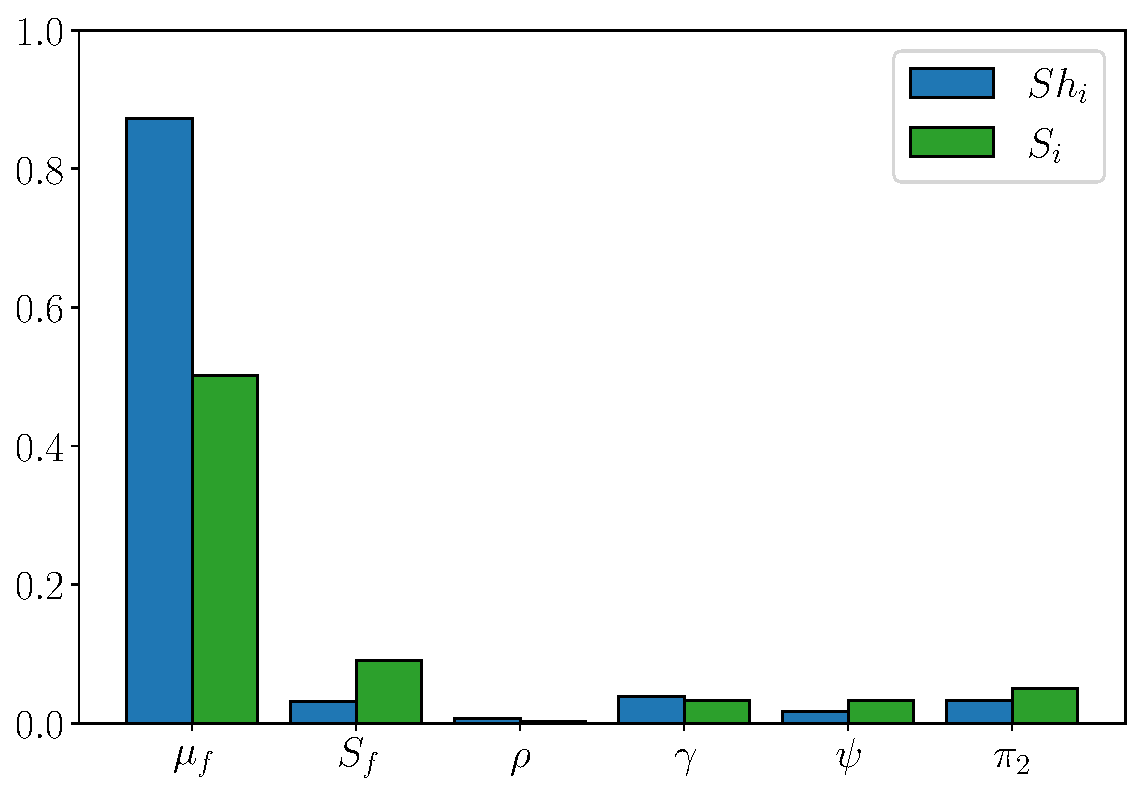
\includegraphics[width=\linewidth]{shapley_S1st_GP_E_scc2100.pdf}

\column{0.49\textwidth}
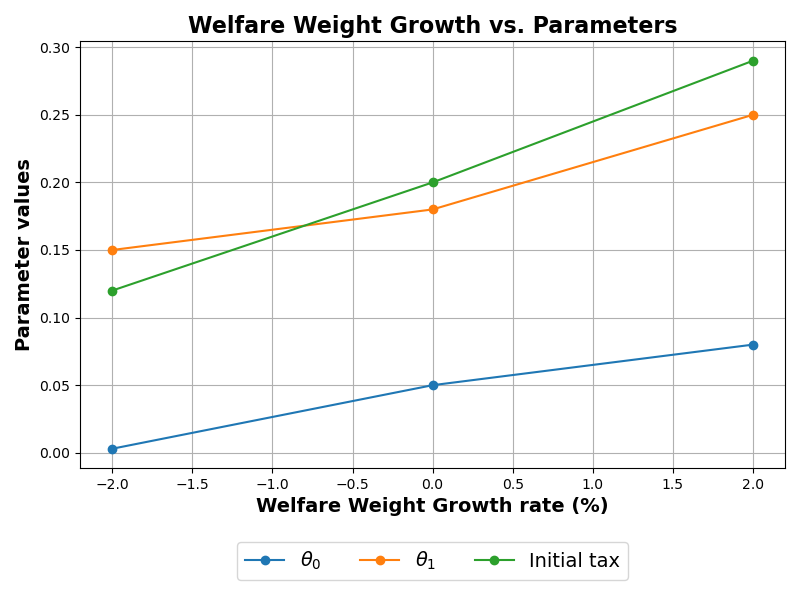
\includegraphics[width=\linewidth]{pareto_frontier_lin_E.png}
\end{columns}

\vspace{0.15cm}
\footnotesize
Left: SCC uncertainty decomposition (Friedl et al., 2023). Right: constrained policy frontier (K\"ubler, Scheidegger \& Surbek, 2026 forthcoming, \emph{J. Political Economy: Macroeconomics}; arXiv:2507.01704).
\end{frame}

% --- Slide 8: Reproducibility checklist ---
\begin{frame}{Implementation Checklist}
\small
\begin{enumerate}
    \item Define state/control vectors and feasibility transforms.
    \item Engineer residual blocks from economics and climate equations.
    \item Set sampling scheme and training diagnostics before tuning architecture.
    \item Validate on out-of-sample simulations and benchmark moments.
    \item Build surrogate/UQ layer only after solver quality is verified.
    \item Separate normative objective from political/participation constraints.
\end{enumerate}
\end{frame}

% --- Slide 9: Frontier directions ---
\begin{frame}{Research Frontier}
\begin{itemize}
    \item Richer heterogeneity: regional, sectoral, and household dimensions.
    \item Endogenous innovation and technology diffusion under climate policy.
    \item Multi-model and model-ensemble learning for robust policy design.
    \item Tight integration of Bayesian learning and policy commitment under ambiguity.
    \item Better theoretical guarantees for convergence and error bounds.
\end{itemize}
\end{frame}

% --- Slide 10: Reading map ---
\begin{frame}{Reading and Notebook Map}
\small
\textbf{Climate readings}
\begin{itemize}
    \item \texttt{readings/links\_by\_lecture/lecture\_16.md} \hfill (CDICE; Folini et al.\ 2025, \emph{Restud})
    \item \texttt{readings/links\_by\_lecture/lecture\_17.md} \hfill (Deep UQ + Pareto carbon tax; KSS 2026 forthcoming, JPE: Macro)
\end{itemize}

\vspace{0.2cm}
\textbf{Climate notebooks} (suggested order)
\begin{itemize}
    \item \texttt{01\_Climate\_Exercise.ipynb} \hfill (NumPy warm-up: carbon cycle, damages, BAU vs mitigation)
    \item \texttt{02\_DICE\_DEQN\_Library\_Port.ipynb} \hfill (deterministic CDICE-DEQN, library port)
    \item \texttt{03\_Stochastic\_DICE\_DEQN.ipynb} \hfill (AR(1) shocks, Gauss--Hermite, SCC fan charts)
\end{itemize}
\end{frame}

% --- Slide 11: Closing ---
\begin{frame}{Closing Message}
\begin{block}{From method to policy}
Deep learning methods are most useful when they improve \emphc{economic credibility},
\emphc{computational scalability}, and \emphc{policy transparency} at the same time.
\end{block}

\vspace{0.5cm}
\begin{center}
{\Large Thank you for participating in the course.}\\[6pt]
{\LARGE \emphc{Questions and discussion}}
\end{center}
\end{frame}

\end{document}
